\documentclass[11pt]{article}
\usepackage{amsfonts}
\usepackage{amsmath}
\usepackage{graphicx}
\usepackage[normalem]{ulem}
\usepackage[a4paper, total={6in, 8in}]{geometry}
\usepackage{listings}
\usepackage{color} %red, green, blue, yellow, cyan, magenta, black, white
\definecolor{mygreen}{RGB}{28,172,0} % color values Red, Green, Blue
\definecolor{mylilas}{RGB}{170,55,241}


\title{Mathematical Modeling HW4}
\author{Miyasaka Kion}
\date{\today}

\begin{document}	
\maketitle

\lstset{language=Matlab,%
    %basicstyle=\color{red},
    breaklines=true,%
    morekeywords={matlab2tikz},
    keywordstyle=\color{blue},%
    morekeywords=[2]{1}, keywordstyle=[2]{\color{black}},
    identifierstyle=\color{black},%
    stringstyle=\color{mylilas},
    commentstyle=\color{mygreen},%
    showstringspaces=false,%without this there will be a symbol in the places where there is a space
    numbers=left,%
    numberstyle={\tiny \color{black}},% size of the numbers
    numbersep=9pt, % this defines how far the numbers are from the text
    emph=[1]{for,end,break},emphstyle=[1]\color{red}, %some words to emphasise
    %emph=[2]{word1,word2}, emphstyle=[2]{style},    
}

\section{Pig Problem}
2. Reconsider the pig problem of Example 1.1, but now suppose that the weight of the pig after $t$ days is $w=800 /\left(1+3 e^{-t / 30}\right)$ lbs.

\


(a) Show that the pig is gaining about $5 \mathrm{lbs} /$ day at $t=0$. What happens as $t$ increases?
\paragraph{Sol.} 
  
Since $w =w=800 /\left(1+3 e^{-t / 30}\right) $, $w' = \frac{80 e^{-\frac{t}{30}}}{\left(3 e^{-\frac{t}{30}}+1\right)^2}$. Hence $w'(0) = 5$.

We can draw a graph of $w$, as below:
\begin{center}
	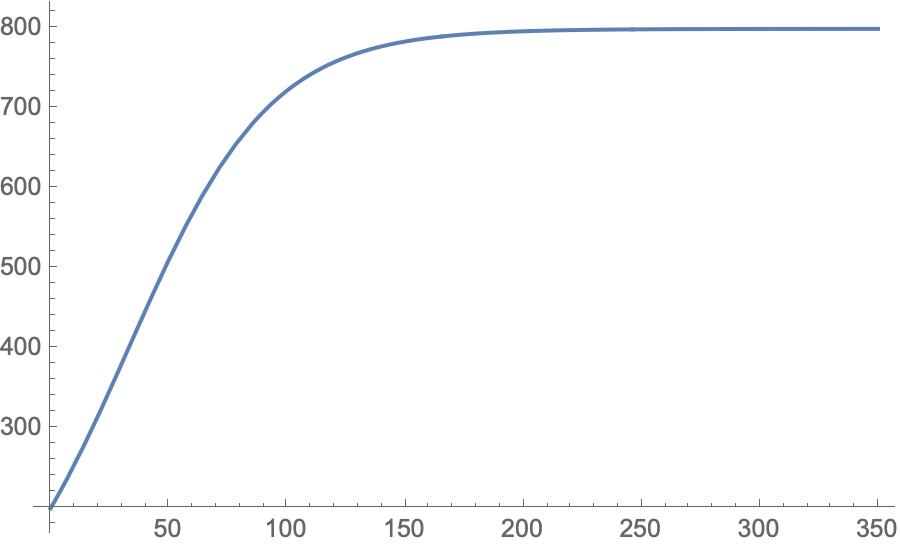
\includegraphics[scale = .5]{pig_1}
\end{center}
This shows that the weight of pig grows relatively rapidly in about the first 150 days, and then keeps nearly the same afterwards.

\

(b) Find the optimal time to sell the pig. Use the five-step approach, and model as a one-variable optimization problem.
\paragraph{Step1.} Ask the question.
$$
\begin{array}{ll}
\text { Variables: } & t=\text { time }(\text { days }) \\
& w=\text { weight of pig }(\mathrm{lbs}) \\
& p=\text { price for pigs }(\$ / \mathrm{lb}) \\
& C=\text { cost of keeping pig } t \text { days }(\$) \\
& R=\text { revenue obtained by selling pig }(\$) \\
& P=\text { profit from sale of pig }(\$) \\
\text { Assumptions: } & w=800 /\left(1+3 e^{-t / 30}\right)\\
& p=0.65-0.01 t \\
& C=0.45 t \\
& R=p \cdot w \\
& P=R-C \\
& t \geq 0 \\
\text { Objective: } \quad & \text { Maximize } P
\end{array}
$$

\paragraph{Step 2.} Select the modeling approach.
This problem can be modeled as a one–variable optimization problem.

\paragraph{Step 3.} Formulate the model.
The objective can be written as
$$
P = R - C = pw - 0.45t = (0.65 - 0.01t)(800/(1+3e^{-t/30})) - 0.45t
$$
i.e.
$$
P(t) = \frac{800 (0.65\, -0.01 t)}{3 e^{-\frac{t}{30}}+1}-0.45 t
$$
\paragraph{Step 4.} Solve the model.

First we can draw a graph and hope we can find some feature of the objective function.

\begin{center}
	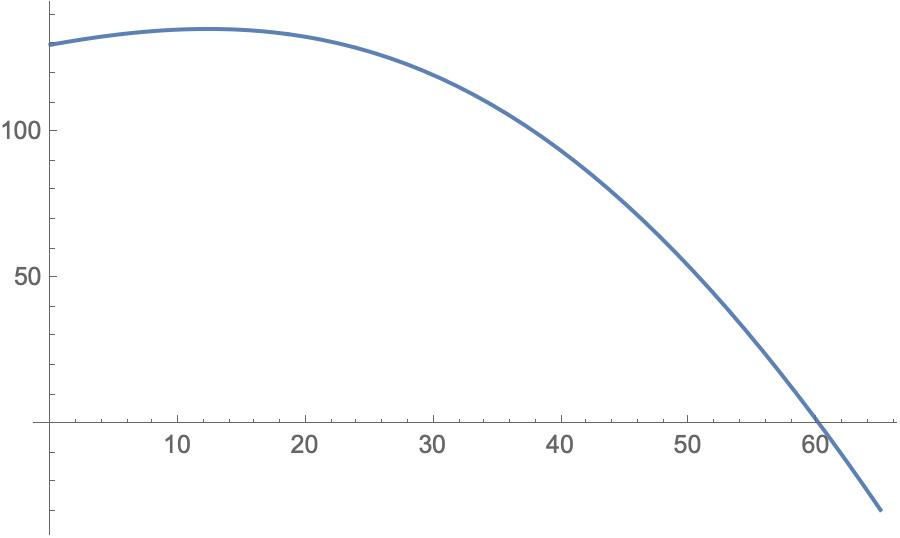
\includegraphics[scale = .5]{HW4_2}
\end{center}

We can obtain that this function is a concave function, at least in $[0,60]$. So if we know where $P' =0$, the maximum point is consequently obtained.
$$
P' = \frac{e^{t/30} (25.3\, -0.8 t)-8.45 e^{t/15}-4.05}{\left(3.\, +e^{t/30}\right)^2}
$$

Then we apply Newton iteration, as the MATLAB code below

\begin{lstlisting}
clear
syms  t f(t) g(t)

f(t) = (0.3E1+exp(1).^((1/30).*t)).^(-2).*((-0.405E1)+(-0.845E1).*exp(1).^((1/15).*t)+exp(1).^((1/30).*t).*(0.253E2+(-0.8E0).*t));
g(t) = diff(f,t);
lt = 0;
for i = 1:200
   newt = double(lt - f(lt)/g(lt));
   if abs(double(lt-newt)) < 0.00001
       break;
   end
   lt = newt;
end
\end{lstlisting}
and the output is $t = 12.3349$ so $P_{\text{max}} = 135.424$ .
% $P_{\text{max}} = \operatorname{max}(P(12), P(13) ) = 135.419\ (t = 12)$.

\paragraph{Step 5.} Answer the question.

If we sell the pig in day $12$, we can obtain the maximum profit of $\$135.419$.

(c) The parameter 800 represents the eventual mature weight of the pig. Perform a sensitivity analysis for this parameter. Consider both the best time to sell and the profit obtained.
\paragraph{Sol.} Replace 800 with L. We first consider the sensitivity of the best time to sell to the const 800.


Then the objective function is 
$$
P= \frac{L (0.65\, -0.01 t)}{3 e^{-\frac{t}{30}}+1}-0.45 t
$$
and it's derivative is
$$
\frac{\mathrm dP}{\mathrm d t} = \frac{e^{t/30} (L (0.035\, -0.001 t)-2.7)+(-0.01 L-0.45) e^{t/15}-4.05}{\left(3.\, +e^{t/30}\right)^2}
$$
When the maximum is reached, there is $\frac{\mathrm dP}{\mathrm d t} = 0$, so put $L$ on the LHS and the other on the RHS, we obtain
$$
L = \frac{-2700. e^{0.0333333 t}-450. e^{0.0666667 t}-4050.}{e^{0.0333333 t} (1. t-35.)+10. e^{0.0666667 t}}
$$
then
$$
S(L,t) = \frac{t \frac{\partial l(t)}{\partial t}}{L} = 2.30978,
$$
$$
S(t,L) = 1/(L,t) = 0.432941.
$$
Hence when $L$ grows $10 \%$, the best selling day $t$ grows by $4.32941\%$.

\subparagraph{Check.} quick check by Mathematica:
\begin{lstlisting}
x = 0.001
p [t_, L_] = (L (0.65` - 0.01` t))/(1 + 3 E^(-t/30)) - 0.45` t
p[12.3349, 800]
( x/12.3349)/((l[12.3349 + x] - l[12.3349])/l[12.3349])
\end{lstlisting}

Output: 0.432853.


  Now we consider the sensitivity of the profit $P$ to the constant 800.
$$
S(P,L) = \frac{\mathrm d P}{\mathrm d L} \cdot \frac{L}{P} \quad \text{where}\quad  L = \frac{-2700. e^{0.0333333 t}-450. e^{0.0666667 t}-4050.}{e^{0.0333333 t} (1. t-35.)+10. e^{0.0666667 t}}
$$




$$
\begin{aligned}
S(P,L) &= \frac{\mathrm d P}{\mathrm d L} \cdot \frac{L}{P} \\
& = \left(\frac{\partial P}{\partial L} + \frac{\partial P}{\partial t}\frac{\mathrm d t}{\mathrm d L}\right)\cdot  \frac{L}{P} \\
& = 
\scalebox{0.7}{%
$\frac{\frac{L e^{-\frac{t}{30}} (0.65\, -0.01 t)}{10 \left(3 e^{-\frac{t}{30}}+1\right)^2}-\frac{0.01 L}{3 e^{-\frac{t}{30}}+1}-0.45}{\frac{-90. e^{0.0333333 t}-30. e^{0.0666667 t}}{e^{0.0333333 t} (1. t-35.)+10. e^{0.0666667 t}}-\frac{\left(-2700. e^{0.0333333 t}-450. e^{0.0666667 t}-4050.\right) \left(0.0333333 e^{0.0333333 t} (1. t-35.)+1. e^{0.0333333 t}+0.666667 e^{0.0666667 t}\right)}{\left(e^{0.0333333 t} (1. t-35.)+10. e^{0.0666667 t}\right)^2}}+\frac{0.65\, -0.01 t}{3 e^{-\frac{t}{30}}+1} \frac{L}{P}$}\\
& =
\scalebox{0.5}{%
$ \frac{e^{0.166667 t} \left(L (0.02 t-0.7)-0.01 t^2+2.5 t-84.25\right)+e^{0.133333 t} \left(L \left(0.002 t^2-0.14 t+2.45\right)+10.8 t-540.\right)+e^{0.1 t} \left(L \left(0.0000666667 t^3-0.007 t^2+0.245 t-2.85833\right)+0.27 t^2-2.7 t-641.25\right)+(0.0666667 L+3.) e^{0.2 t}+e^{0.0666667 t} \left(0.54 t^2-37.8 t+418.5\right)}{\left(3.\, +e^{t/30}\right)^2 \left(e^{0.0333333 t} (45.\, -9. t)+e^{0.1 t} (1. t-125.)-360. e^{0.0666667 t}\right)}  \frac{L}{P}$}\\
&  = 1.04099,
\end{aligned}
$$



which means if L grows by 10\%, the profit will also grow by 10.4099\%.

\subparagraph{Check.} quick check by Mathematica:
\begin{lstlisting}
x = 0.0001
((p[12.3349, 800 + x] - p[12.3349, 800])/p[12.3349] )/(x/800)
\end{lstlisting}

Output: 1.04099

\section{Facility location problem}
6. Reconsider the facility location problem of Example $3.2$, but now assume that the response time from point $\left(x_{0}, y_{0}\right)$ to point $\left(x_{1}, y_{1}\right)$ is proportional to the road travel distance $\left|x_{1}-x_{0}\right|+\left|y_{1}-y_{0}\right|$.
(a) Find the location that minimizes average response time. Use the five-step method, and model as a multivariable unconstrained optimization problem.
\paragraph{Step 1.} Ask the question.

$$
\begin{array}{ll}
\text { Variables: } 
& d = \text{distance between the dweller and the facility(mile(s))}\\
& T = \text{total time cost(minute(s))} \\
\text { Assumptions: } 
& x_i,y_i \quad \text{are given in figure in the text book}\\
& r_i(x,y) = |x-x_i| + |y-y_i| \\
& t(d_i) =   3.2 + 1.7r_i ^{0.91}\\
& T = \sum t(r_i) \\
\text { Objective: } \quad & \text { Minimize } T
\end{array}
$$

 \paragraph{Step 2.} Select the modeling approach.
 
 We treat this problem as a single variable constrained optimization problem.
 
\paragraph{Step 3.} Formulate the model.

$$
\begin{aligned}
&0.0202381\left(8(|x-5|+|y-5|)^{0.91}+8(|x-3|+|y-5|)^{0.91}+\right. \\
&6(|x-1|+|y-5|)^{0.91}+3(|x-5|+|y-3|)^{0.91}+ \\
&6(|x-3|+|y-3|)^{0.91}+21(|x-1|+|y-3|)^{0.91}+ \\
&6(|x-5|+|y-1|)^{0.91}+8(|x-3|+|y-1|)^{0.91}+ \\
&18(|x-1|+|y-1|)^{0.91}+3.2
\end{aligned}
$$

\paragraph{Step 4.} Solve the model.

We can use random search to approximate an optimal solution.

\begin{lstlisting}
clear 
syms x y f(x,y,a,b) z(x,y)
f(x,y,a,b) = (abs(x-a)+abs(y-b))^0.91;
z(x,y) = 3.2+1.7*( 6*f(x,y,1,5) + 8*f(x,y,3,5) + 8*f(x,y,5,5) + 21*f(x,y,1,3) + 6*f(x,y,3,3) + 3*f(x,y,5,3) +18*f(x,y,1,1) + 8*f(x,y,3,1) + 6*f(x,y,5,1))/84;
% z(x,y) = simplify(z(x,y));
range_y = [0 6];
range_x = range_y;
INF = 0x7fffffff;
N = 0;
sz = [1 2];
zmin = INF;
minx = -INF;
miny = -INF;
std_ans = 6.46298;
A = [];
N = 50000;
   
for i = 1:N
   cx = (range_x(2) - range_x(1)) * rand + range_x(1);
   cy = (range_y(2) - range_y(1)) * rand + range_y(1);
   cz = double(z(cx,cy));
   if cz < zmin 
       zmin = cz;
       xmin = cx;
       ymin = cy;
   end      
end
[xmin, ymin, zmin]
\end{lstlisting}

The output is $x = 1.0121 , y =   3.0062 $ and $ T =   7.1559$, as a lucky enough guy, simply suppose that $ x = 1$ and $ y = 3$ we have $T = 7.14535$ which is absolutely smaller then the value we got.
We can then apply the gradient descent method on the basis of the previous result, we start searching the optimal solution from  $x = 1.0121 , y =   3.0062 $ in the precision of $0.0001$(Mathematica):

\begin{lstlisting}
Clear[x, y, a, b, T, f, t, dt, beta]
f[x_, y_, a_, b_] = (Sqrt[(x - a)^2] + Sqrt[(y - b)^2])^0.91;
T[x_, y_] = 
  3.2 + 1.7*(6*f[x, y, 1, 5] + 8*f[x, y, 3, 5] + 8*f[x, y, 5, 5] + 
       21*f[x, y, 1, 3] + 6*f[x, y, 3, 3] + 3*f[x, y, 5, 3] + 
       18*f[x, y, 1, 1] + 8*f[x, y, 3, 1] + 6*f[x, y, 5, 1])/84;
dt[x_, y_ ] = Simplify[Grad[T[x, y], {x, y}]];
beta = 0.00001;
f[{x_, y_}] = {x, y} - beta*Grad[T[x, y], {x, y}];
Nest[f, {1.0121, 3.0062}, 1000000]
\end{lstlisting}
 and the output is $1.0000099190304728`, 2.9999979259962877$, i.e. $x = 1.0000099190304728, y = 2.9999979259962877$ and $T = 7.14536$ which is still larger then the value we guessed.
 
Since the precision of the answer is precise enough, we can simply just pick the answer $x = 1,y = 3$ and $T = 7.14535$ as the final result.
\paragraph{Step 5.} Answer the question.
In order to minimize the time to reach any dweller in the district, the facility build at (1,3) is optimal, and the time is 7.14536 minutes.


 


\end{document}